\part{III: Gaps, Gluts, and Propagation}\label{part-iii-gaps-gluts-and-propagation}

\hypertarget{chapter-9-gaps-determination-without-bivalence}{%
\chapter*{Chapter 9 --- Gaps: Determination Without Bivalence}
\addcontentsline{toc}{chapter}{Chapter 9 --- Gaps: Determination Without Bivalence}
\markboth{Chapter 9 --- Gaps: Determination Without Bivalence}{Chapter 9 --- Gaps: Determination Without Bivalence}\label{chapter-9-gaps-determination-without-bivalence}}

Chapter 2 argued that distinction precedes truth: before a proposition
can be true or false, something has to be carved out as a determinate
content for a truth value to apply to. This chapter takes the next step,
and it's a smaller one than it might look: once truth values are read off
evidence rather than assumed in advance, the possibility that evidence is
simply \emph{absent} has to be taken seriously as its own case, not folded
into ``false'' or treated as a defect.

\textbf{Two independent questions, minimally.} Ask, of a proposition \(p\): is
there positive support for \(p\) --- evidence, a witness, a derivation, in
whatever sense support is available in the context at hand? And,
separately: is there negative support for \(p\)? Nothing forces these two
questions to have correlated answers. A failure to find positive support
does not, by itself, hand you negative support --- the absence of a reason
to affirm something is not a reason to deny it. That's not a special
principle needing independent defense; it's simply what it means for the
two questions to be genuinely two questions rather than one question
asked twice.

\textbf{What underdetermination is, and isn't.} When neither kind of support
is present, call \(p\) \textbf{underdetermined} at that context. This is not a
third truth value smuggled in alongside true and false --- it's what ``no
answer to either question yet'' already amounts to, once the two
questions have been separated. Priest's own examples fit cleanly here
without needing modification: a definite description with no referent
(``the current King of France is bald'') supplies neither positive nor
negative support for predications about its subject, because there's no
subject there to support anything about. A future contingent --- a claim
about tomorrow's sea battle, asked today --- has no positive support (the
battle hasn't happened) and, importantly, no negative support either (its
non-occurrence hasn't happened yet), which is a different situation from
a claim that has been actively falsified.

\textbf{Why a gap is not an obstruction.} This is the point worth stating
carefully, because it will matter again once Part VI generalizes this
material: underdetermination is harmless in a specific, checkable sense.
An underdetermined proposition imposes no obstacle to reconstructing a
larger picture around it --- you can always extend an underdetermined case
with more information later, in either direction, without having to
retract anything you'd previously committed to, because you hadn't
committed to anything yet. A gap doesn't need repairing; it needs
filling in, which is a different operation with a different cost. That
distinction --- between a state that costs nothing to extend and a state
that actively resists coherent extension --- is what separates this
chapter from the next one, and conflating them is the single most common
way nonclassical semantics gets misread as a uniform tolerance for
``weirdness,'' when in fact gaps and gluts are opposite kinds of case, not
two flavors of the same thing.

\hypertarget{chapter-10-gluts-contradiction-as-retained-information}{%
\chapter*{Chapter 10 --- Gluts: Contradiction as Retained Information}
\addcontentsline{toc}{chapter}{Chapter 10 --- Gluts: Contradiction as Retained Information}
\markboth{Chapter 10 --- Gluts: Contradiction as Retained Information}{Chapter 10 --- Gluts: Contradiction as Retained Information}\label{chapter-10-gluts-contradiction-as-retained-information}}

Chapter 9 established that absence of support in one direction doesn't
force support in the other. This chapter is about what happens when both
directions are actually supported at once --- and argues that the right
response is not automatically to treat this as an error state requiring
correction.

\textbf{The four statuses, from two coordinates.} With both positive and
negative support now genuinely in play, the same construction from
Chapter 9 yields four cases rather than two: no support either way
(underdetermined, Chapter 9's subject), positive support only, negative
support only, and --- the new case --- both. Call a proposition with both
positive and negative support \textbf{overdetermined}. This is Belnap and
Dunn's~\cite{belnap1977,dunn1976} fourth value, arrived at the same way the other three were: as a
consequence of what the support data actually contains, not as a
stipulated addition to a prior two-valued base.

\begin{figure}[htbp]
\centering
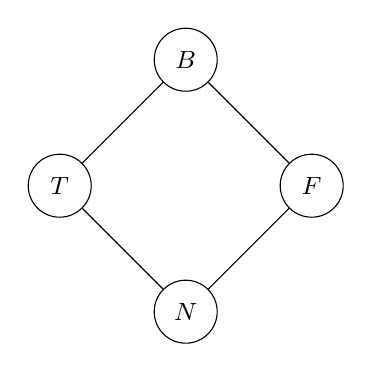
\begin{tikzpicture}[
  node distance=1.6cm and 1.6cm,
  val/.style={draw, circle, minimum size=8mm, inner sep=0pt, font=\small},
  lbl/.style={font=\footnotesize, midway, sloped}
]
\node[val] (B) at (0,1.6) {$B$};
\node[val] (T) at (-1.6,0) {$T$};
\node[val] (F) at (1.6,0) {$F$};
\node[val] (N) at (0,-1.6) {$N$};
\draw (N) -- (T);
\draw (N) -- (F);
\draw (T) -- (B);
\draw (F) -- (B);
\end{tikzpicture}
\caption{The Belnap--Dunn information lattice $\mathbb{F} = \{N,T,F,B\}$
under the information order $\sqsubseteq_k$. $N$ is bottom (no support),
$B$ is top (both polarities), and $T,F$ are incomparable. Consequently
$T \vee_k F = B$: pooling positive-only and negative-only support
produces a glut by construction, not by exception.}
\label{fig:belnap-lattice}
\end{figure}

\textbf{The claim that matters is stronger than ``some propositions are both
true and false.''} That phrasing makes overdetermination sound like a
metaphysical oddity --- a strange fact about certain propositions. The
sharper claim is procedural: contradictory evidence does not need to be
\emph{deleted} merely because it is contradictory. Given two conflicting
bodies of evidence, a system has a choice about what to do with the
conflict, and ``erase one side'' is only one option among several, not the
obviously correct one. Chapter 4's refusal machinery is exactly what
makes the alternative precise: a regime can \emph{refuse} the deletion ---
decline, as a constitutive matter, to treat ``these conflict'' as
sufficient grounds for discarding either witness --- and retain both. That
refusal is not indecision or error-tolerance. It's a principled
commitment to not letting a specific kind of local conflict force a loss
of information that nothing yet justifies losing.

\textbf{What this is not.} Overdetermination is not the same epistemic
situation as uncertainty. ``We don't know whether \(p\)'' is Chapter 9's
underdetermination --- absence of support in both directions.
``We have positive and negative support for \(p\)'' is a different fact
entirely --- presence of support in both directions --- and treating the two
as interchangeable (as ordinary language sometimes does, calling both
situations ``unclear'') erases a distinction the rest of this book depends
on. Priest's semantic paradoxes (the Liar sentence, under a sufficiently
expressive language, genuinely supports both its own truth and its own
falsity by the ordinary rules governing truth predicates), and the
existence of legal and normative systems that contain live, unresolved
contradictions without therefore becoming useless, are both cases of
overdetermination in this sense, not cases of not-yet-knowing.

\textbf{The asymmetry, stated once, philosophically, ahead of its formal
treatment.} Chapter 9's gaps and this chapter's gluts are not mirror
images of each other, whatever the symmetry of the four-value notation
suggests. A gap costs nothing and obstructs nothing; it is the default,
harmless case. A glut is the substantive case --- the one that actually
requires the rest of this book's machinery to handle responsibly. Part
VI gives this asymmetry an exact formal statement; here it is enough to
notice that ``insufficient support'' and ``incompatible support'' are not
symmetric failures, and treating them as if they were is a mistake this
book avoids from the outset rather than discovering later.

\hypertarget{chapter-11-paraconsistency-why-contradiction-does-not-propagate}{%
\chapter*{Chapter 11 --- Paraconsistency: Why Contradiction Does Not Propagate}
\addcontentsline{toc}{chapter}{Chapter 11 --- Paraconsistency: Why Contradiction Does Not Propagate}
\markboth{Chapter 11 --- Paraconsistency: Why Contradiction Does Not Propagate}{Chapter 11 --- Paraconsistency: Why Contradiction Does Not Propagate}\label{chapter-11-paraconsistency-why-contradiction-does-not-propagate}}

Chapter 4 separated inconsistency from triviality and left one question
open: what has to be true of a system's propagation rules for the
former not to become the latter? This chapter answers it, and it is the
technical centerpiece of Part III.

\textbf{Explosion as one specific propagation rule, not a logical necessity.}
Classically, from \(p\) and \(\neg p\), anything follows --- most directly via
disjunctive syllogism: from \(p \vee q\) and \(\neg p\), infer \(q\); since \(p\)
is available, \(p \vee q\) holds for any \(q\) whatsoever, and \(\neg p\) is
also available, so \(q\) follows, for arbitrary \(q\). Every step in that
derivation is individually classically valid. The question this chapter
asks is not whether the derivation is classically valid --- it is --- but
whether a system is \emph{obligated} to make disjunctive syllogism available
at a point where both \(p\) and \(\neg p\) are independently supported.

\textbf{Why the answer can be no, without giving up inference generally.}
Consider a proposition \(p\) that is overdetermined --- both \(p\) and \(\neg p\)
supported, in Chapter 10's sense. Disjunctive syllogism, applied here,
uses the \emph{positive} support for \(p\) to license \(p \vee q\), and then uses
the \emph{negative} support for \(p\) (i.e., \(\neg p\)) to discharge the \(p\)
disjunct and leave \(q\) standing --- treating the negative support as if it
straightforwardly eliminated the positive support's contribution. But
that is exactly the move Chapter 10 argued a system need not make: the
negative support doesn't erase the positive support in an overdetermined
case, by definition --- that's what overdetermination \emph{is}. Disjunctive
syllogism's second step silently assumes the positive and negative
supports can't coexist, which is precisely false at an overdetermined
point. Blocking disjunctive syllogism at exactly these points is not an
ad hoc patch to avoid an unwanted conclusion; it's the direct consequence
of taking Chapter 10's retained-information picture seriously rather than
only in the abstract.

\textbf{The general propagation principle.} Stated once, for use throughout
the rest of the book: a local failure should propagate only as far as
the dependency structure connecting it to other propositions actually
warrants --- not automatically to every proposition in the language, which
is what unrestricted closure (Chapter 3) does by default. Restricting
propagation at exactly the step that assumes what an overdetermined
proposition specifically denies is what keeps a contradiction local. This
is also why paraconsistency is not ``logic with the brakes cut'' --- if
anything, it's the more conservative regime: it declines to license an
inferential step whose validity depended on an assumption (that positive
and negative support are mutually exclusive) that the very situation
under discussion has already falsified.

\hypertarget{chapter-12-repair-and-classical-recapture}{%
\chapter*{Chapter 12 --- Repair and Classical Recapture}
\addcontentsline{toc}{chapter}{Chapter 12 --- Repair and Classical Recapture}
\markboth{Chapter 12 --- Repair and Classical Recapture}{Chapter 12 --- Repair and Classical Recapture}\label{chapter-12-repair-and-classical-recapture}}

Part III closes by asking what a system should actually \emph{do} once it
has an overdetermined proposition on its hands, rather than merely
tolerating its presence.

\textbf{The merge.} Given several independent bodies of evidence
\(s_1, \dots, s_n\) bearing on \(p\) --- not yet organized spatially into
patches or a cover, simply distinct sources --- their combination is given
by the pointwise information merge
\[M(p) = \bigvee_i s_i(p),\]
the least assignment that retains everything each source individually
supplied. This always exists (no combination of sources can fail to have
a merge), and \(M(p)\) comes out overdetermined exactly when the sources
collectively supply both positive and negative support for \(p\) --- which
is precisely Chapter 10's notion, arrived at now as a consequence of
combining evidence rather than stipulated about a single source.

\textbf{Why the classical alternative genuinely fails, rather than merely
being undesirable.} Suppose a system insists on a glut-free
reconstruction --- a single, classical assignment of true-or-false to \(p\)
that's consistent with everything the sources supplied. If the sources
jointly supply both positive and negative support, no such assignment
exists: anything siding with the positive evidence contradicts the
negative evidence, and vice versa. This is a genuine non-existence
result, not a preference --- a classical, no-glut regime has \emph{no}
admissible reconstruction of that evidence at all. Paraconsistency's
contribution here is not ``tolerating an error the classical approach
would have caught.'' It's supplying a reconstruction --- \(M(p) = B\) --- where
the classical regime supplies none. The paraconsistent regime has
strictly more admissible outcomes available to it, and this is one of
them being used, not an error being excused.

\textbf{Classical recapture.} A system that admits overdetermination
everywhere it's forced to, but nowhere else, and actively minimizes how
much of the language ends up overdetermined, recovers classical behavior
almost everywhere while preserving exactly the local gluts the evidence
actually demands --- this is Priest's minimally inconsistent LP, and in
this book's vocabulary it is a repair operator biased toward
consistency: pay the cost of a glut only where the evidence leaves no
alternative, default to classical, glut-free assignment everywhere else.
This is the first appearance, at the level of a single proposition and
its sources, of a idea Part VI will generalize considerably: repair is
not the opposite of classical reasoning, it's classical reasoning with an
escape hatch for the specific cases where classical reasoning has
nowhere to go.

\textbf{The arc of Part III, and what it deliberately withholds.} Chapters
9--12 trace one continuous line: underdetermination, independent support,
overdetermination, restricted propagation, repair. Everything in this
arc is local and order-theoretic --- a fact about single propositions and
the evidence bearing on them, not about how evidence distributed across
many regions of a larger structure does or doesn't cohere with itself.
That second question --- what happens once these support objects are
localized over a genuine cover, and whether local overdetermination has
anything to do with whether the pieces of evidence agree with each other
in the first place --- is Part VI's question, not this one's, and this
part has deliberately not reached for it. Cohomology, coherence defects,
and the distinction between a glut and an obstruction to gluing are held
back on purpose: introducing them here would answer Part VI's question
before its own machinery exists to ask it properly, and would blur
exactly the local/global independence that turns out to be one of this
book's more original claims.

\hypertarget{status-of-this-draft}{%
\section{Status of this draft}\label{status-of-this-draft}}

Written to be self-contained: a reader who stops after Part III has a
complete, correct account of gaps, gluts, paraconsistency, and repair at
the level of individual propositions and their evidence, without needing
anything from Part VI. Deliberately withheld throughout: any mention of
covers, patches, coherence defects, or cohomology --- those are held for
Part VI specifically so that Part III's account doesn't accidentally
answer, or foreclose, the question of whether local nonclassical
valuation and global structural obstruction are related. One thing to
verify once Part VI is revised last (per the drafting order settled on):
that Chapter 12's merge proposition and Part VI's Chapter 21 restatement
of the same result are stated compatibly, since they're now the same
claim appearing at two different levels of generality and any drift
between the two would be worth catching before either is called final.
